\documentclass[12pt]{article}

\usepackage[margin=1in]{geometry}  % set the margins to 1in on all sides
\usepackage{graphicx}              % to include figures
\usepackage{amsmath}               % great math stuff
\usepackage{amsfonts}              % for blackboard bold, etc
\usepackage{amsthm}                % better theorem environments
\usepackage{bm}					   % bm for bold math

\usepackage{enumitem} % for [noitemsep]
\usepackage{rotating} % for sideway table
\usepackage{caption} % for newline in caption
\usepackage{xcolor}
\usepackage{hyperref}
\hypersetup{
    colorlinks,
    linkcolor={red!50!black},
    citecolor={blue!50!black},
    urlcolor={blue!80!black}
}
\usepackage{cleveref}

\usepackage{array,tabularx}
  
\usepackage{float}
\restylefloat{table}

% bibliography
\usepackage{natbib}
\bibpunct{(}{)}{;}{a}{}{,} % no comma between author and year

\title{The political determinants of FDI spillover}
\author{Anh Le}


\begin{document}
\maketitle

\section{Introduction}
\label{sec:introduction}

The political science literature on Foreign Direct Investment (FDI) has focused largely on how politics shapes the flow of FDI across countries. The central insight of this literature is that multinational corporations (MNCs) face an ``obsolescing bargain'' against the host government. Once the MNC has sunk its investment, it is vulnerable to the host government's changing regulations, backtracking on deals, or even expropriating its properties \citep{Li2009a, Sawant2010}. Certain institutional and political characteristics, such as numerous veto players, executive constraint, or strong property rights, allow the host government to make a credible commitment and thus ameliorate the severity of the ``obsolescing bargain'' problem \citep{Busse2007, Jensen2014, Li2003}. According to the literature, MNCs should invest more in countries with these characteristics.

This dominant approach in the literature has three long-standing issues that my paper will address. First, the majority of the literature relies on FDI stock and flow data as the outcome of interest even though they are often not an appropriate measure for the scale of MNCs' activities \citep{Kerner2014}. While it would be ideal to use firm-level data instead, both the lack of cross-national firm-level data and a suitable statistical model have posed a challenge.

Second, while there has been much focus on MNCs choosing host countries, the literature has largely neglected the other side of the investment decision: what are countries' preferences regarding MNCs? Consider the established finding that democracies receive more FDI. Without controlling for countries' preferences, it is difficult to interpret this fact as democracies actively pursuing MNCs or as MNCs finding democracies attractive. Not only are countries' preferences central to the modeling of investment decision, arguably it is also more steeped with politics and deserves more attention. \citet{Pinto2013} and \citet{Pandya2016} are two pioneering works in this area of research, proposing partisan politics and regime types as factors shaping countries' preferences for FDI. However, while their theories are ground-breaking, the empirical estimation of countries' preferences remains difficult.

Third, in addition to empirical issues raised above, I propose that we need to theorize about countries' preferences for FDI quality. While the political science literature has largely focused on the quantity of FDI, national policies and discourses pay much attention to the quality of FDI, using various incentives and restrictions to target certain types of FDI. Indeed, MNCs come with varying capital, demand for labor, and technology, all of which have different effects on the host country's economy. For example, policy makers and scholars have highlighted high-tech MNCs as a source of technological transfer for developing host countries, allowing them to upgrade their technical capacity and improve their productivity \citep{Findlay1978, Nunnenkamp2004}. While such high-quality FDI has been enthusiastically endorsed by the development community, I argue that only governments with a long time horizon want to attract high-tech FDI because technological transfer takes time to pay off.

In sum, the current literature would benefit from an analysis that is capable of using firm-level data to estimate both firms' and countries' preferences for each other's characteristics. To accomplish this goal, I adapt the two-sided matching model originally designed for the labor market and the marriage market. In this model, both firms and countries evaluate their available options and choose the best according to their utility functions. As in many social science contexts, we only observe the final firm-country matches and not the full set of available options (also known as the opportunity set). I solve this problem by using the Metropolis Hastings algorithm, a Markov chain Monte Carlo (MCMC) approach that repeatedly samples new opportunity sets and rejects them at an appropriate rate to approximate their true distribution. Since the two-sided matching model is derived explicitly from actors' utility functions, their parameters also enjoy a straightforward interpretation in the utility space instead of some aggregate outcomes.

The paper proceeds as follows. \Cref{sec:literature_issues} discusses the three long-standing issues with the literature and how they can be improved. \Cref{sec:model} lays out the utility structure in the two-sided matching model and describes the matching process. \Cref{sec:tsl_estimate} shows how the model can be estimated with the Metropolis-Hastings algorithm. \Cref{sec:application} shows an application of the model on a census of Japanese firms overseas. \Cref{sec:result} presents the result. \Cref{sec:conclusion} concludes.

\section{Literature}


1. FDI aggregate data is not clear about what it means to be foreign. IMF decides 10\% is the line between foreign portfolio investment and FDI

\section{The Two-Sided Matching Model}
\label{sec:model}

\subsection{Officials' Utility}

Following \citet{Logan1998}, we consider the utility function of two actors, the official and the firm.\footnote{For ease of exposition, in this section I will refer to country $j$ and official $j$ interchangeably.} For official $j$, the utility of having firm $i$ investing in his country is:

\begin{align}
U_j(i) &= \bm{\beta}_j' X_i + \epsilon_{1ij}
\end{align}

where

\begin{align*}
\beta_j &\text{ is a vector of official $j$'s preference for relevant characteristics of firms} \\
x_i &\text{ is a vector of firm $i$'s measured values on those characteristics} \\
\epsilon_{1ij} &\text{ is the unobserved component that influences official $j$'s utility}
\end{align*}

On the other hand, the utility of not having firm $i$ investing is:

\begin{align}
U_j(\neg i) &= b_j + \epsilon_{0ij}
\end{align}

where

\begin{align*}
b_j &\text{ is the baseline utility of official $j$ without any firm investing} \\
\epsilon_{0ij} &\text{ is the component that influences official $j$'s utility}
\end{align*}

For each firm $i$, official $j$ will make an offer to invest if $U_j(i) > U_j(\neg i)$. Relevant firm characteristics (i.e. $X_i$) that the official may consider are: technological intensity, number of jobs, and size of capital. The corresponding $\beta$'s represent the official's preference for these characteristics.

Following the discrete choice literature, we model $\epsilon_{1ij}, \epsilon_{0ij}$ as having the Gumbel distribution. Then, the probability of official $j$ making an offer to firm $i$ takes the familiar binomial logit form:

\begin{align}
Pr(o_{ij} = 1) &= Pr(U_j(i) > U_j(\neg i)) \\
&= Pr(\epsilon_{0ij} - \epsilon_{1ij} <  \bm{\beta}_j ' X_i - b_j) \\
&= \frac{\exp({\bm{\beta}_j'X_i})}{1 + \exp({\bm{\beta}_j'X_i})} \label{eq:prob_offer_ij}
\end{align}

where \Cref{eq:prob_offer_ij} is due to the fact that the difference between two Gumbel-distributed random variables has a logistic distribution. We make the constant term $b_j$ disappear into $\bm{\beta}_j$ by adding an intercept column to the matrix of firm characteristics $X_i$.

The opportunity set of firm $i$ is the set of all countries that welcomes firm $i$ to invest. If we know the preferences of all countries, we can calculate the probability that firm $i$ gets an opportunity set $O_i$ as follows:

\begin{align}
p(O_i | \bm{\beta}) &= \prod_{j \in O_i} p(o_{ij} = 1 | \bm{\beta}) \prod_{j \notin O_i} p(o_{ij} = 0 | \bm{\beta}) \\
&= \prod_{j \in O_i} \frac{\exp(\bm{\beta_j} ' X_i)}{1 + \exp(\bm{\beta_j}' X_i)}
 \prod_{j \notin O_i} \frac{\exp(\bm{\beta_j} ' X_i)}{1 + \exp(\bm{\beta_j}' X_i)} \label{eq:conditional_probability_of_offer}
\end{align}

In our observed data, since we only observe the final matching of firms and countries, this opportunity set is unobserved. As \Cref{sec:tsl_estimate} will discuss, we use the Metropolis-Hastings algorithm to sample from and approximate $p(O_i | \bm \beta)$.

\subsection{Firms' utility}

On the other side, for firm $i$, the utility of investing in country $j$ is:

\begin{align}
V_i(j) &= \alpha' W_{j} + v_{ij}
\end{align}

where

\begin{align*}
\alpha &\text{ is a vector of firms' preference for relevant characteristics of countries} \\
W_j &\text{ is a vector of country $j$ measured values on those characteristics} \\
v_{ij} &\text{ is the unobserved component that influences firm $i$'s utility}
\end{align*}

Firm $i$ evaluates all the countries that welcome it to invest and chooses the country that brings the highest utility. In our model, relevant country characteristics can be: labor quality, level of development, and market size. Since all firms are considered having homogeneous preferences, $\alpha$ does not have a subscript $i$. The model can be easily extended so that there is heterogeneous preference among firms.

If $v_{ij}$ is modeled as having a Gumbel distribution, then the probability that firm $i$ will accept the offer of official $j$ out of all the offers in its opportunity set $O_i$ takes the multinomial logit form \citep{Cameron2005}:

\begin{align}
p(A_i = a_i | O_i, \alpha_i) = \frac{\exp(\alpha'W_{a_i})}{\sum\limits_{j:j \in O_i} \exp(\alpha'W_j)} \label{eq:conditional_probability_of_accept}
\end{align}

\section{Model Estimation}
\label{sec:tsl_estimate}

While \citet{Logan1996, Logan1998} successfully reformulate the random utility mode in the discrete choice literature to a two-sided setting, the estimation of the two-sided model remains challenging. The key difficulty lies in the fact that we do not know the full sets of offers that firms receive from countries. Therefore, the likelihood function is incomplete, missing the data on firms' opportunity sets. With an incomplete likelihood function, we cannot use Maximum Likelihood Estimation to estimate firms' and countries' preferences.

To solve this problem, \cite{Logan1996} uses the Expectation-Maximization (EM) algorithm.\footnote{The EM algorithm finds the best parameter estimates by iterating between two steps. First, given the current best guess of firms' and countries' preferences, pick values for the unobserved opportunity sets so that we maximize the likelihood. Second, given the current best guess of the unobserved opportunity sets, taken from step 1, pick values for firms' and countries' preferences so that we maximize the likelihood. By iterating between these two steps, the algorithm constantly searches for parameters values that maximize the likelihood.} However, an important downside of the EM algorithm is its lack of standard error. Therefore, while the algorithm is capable of producing the best estimate for the parameters of interest, it is difficult to know how good our best guess really is.

To overcome this difficulty, I use the Metropolis-Hastings algorithm, a MCMC approach that can approximate the posterior distribution of the opportunity sets, firms' and countries' preferences.

For example, we want to sample from the posterior distribution of the opportunity sets, $p(O|\text{data})$, which can take any complicated form. Suppose we already had a working collection of values $\{O^{1}, \dots, O^{(s)}\}$. To add new values to this collection, we would propose a new value $O^*$, then decide whether to keep it with the probability $\frac{p(O^*|\text{data})}{p(O|\text{data})}$. The intuition is that if $\frac{p(O^*|\text{data})}{p(O|\text{data})}$ is large, then $O^*$ is very likely compared to $O$ given $p(O|\text{data})$. Thus, we should keep $O^*$ and add it to the collection. In other words, we decide to keep newly proposed values of $O$ at a rate proportional to how often they should appear according to $p(O|\text{data})$. Repeating this step many times, at the end we will have a collection of $O$ values that approximates $p(O|\text{data})$ as desired.

\Cref{appendix:MH_ratio} describes the details of our model estimation and derives the Metropolis-Hastings acceptance ratio. I use flat priors so that our results are driven entirely by the data. In deriving the joint distribution of the data and parameters, including the opportunity sets, the firms' and countries' preferences, there are two important ideas. First, the opportunity sets are determined solely by countries' preferences, not firms'. Second, given the opportunity sets, the final matches are determined solely by firms' preferences, not countries'. Thus, the joint distribution of data and parameters factors out nicely as follows:

\[
p(A_i, O_i, \alpha, \bm{\beta}) = p(A_i|O_i, \alpha) p(O_i | \bm{\beta})
\]

where $A_i$ denotes the country that firm $i$ accepts to invest in, i.e. the observed match data.


My data use capital size, which is great because that's exactly what countries look for. 


\citep[295]{Yamawaki1991} says that the data ``list virtually all the foreign subsidiaries of Japanese companies''

\section{Results}
\label{sec:result}

We run a Metropolis-Hastings algorithm for 2,000,000 iterations. To reduce autocorrelation between iterations, we thin the sample and only keep the sampled values every 100 steps, resulting in a final posterior sample of 20,000.

\subsection{Results on Firms' Preferences}

\Cref{fig:traceplot_alpha} show the trace plots of $\alpha$, firms' preference parameters for countries' log GDP, log GDP per capita, democracy, and labor quality. The plots show that the MCMC chains do converge after the 5000\textsuperscript{th} iterations with the exception of the preference parameter for log GDP per capita. Our interpretation of this parameter is therefore more speculative.

\begin{figure}[!ht]
\centering
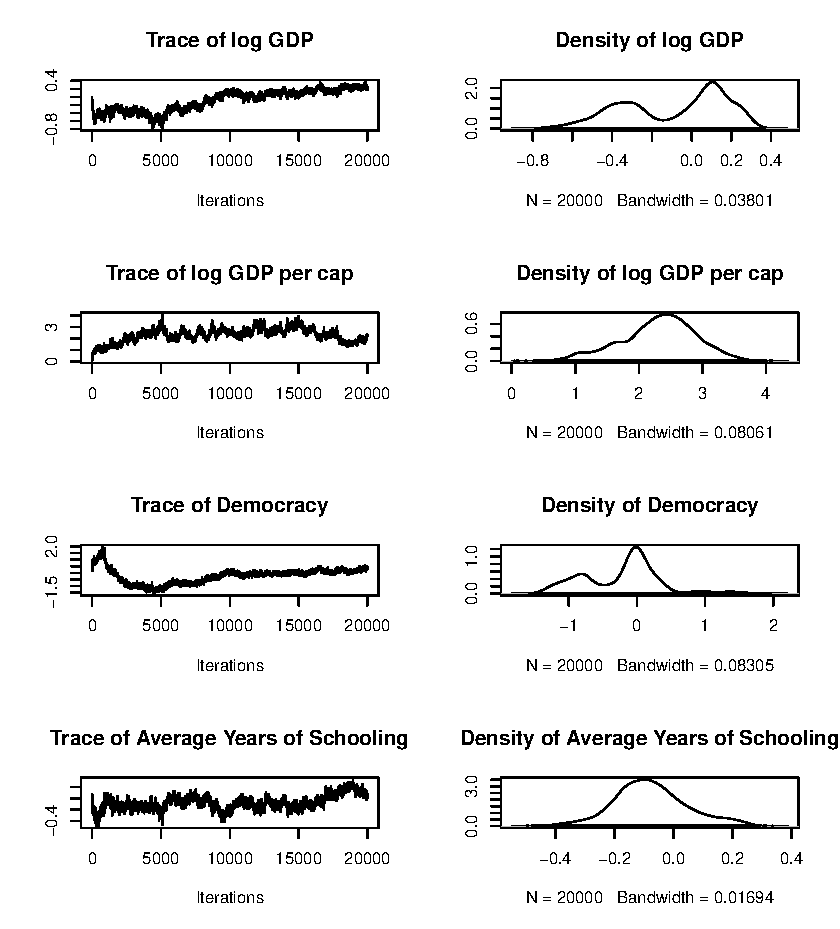
\includegraphics[width=\textwidth,keepaspectratio]{../figure/traceplot_alpha}
\caption{Traceplot.}
\label{fig:traceplot_alpha}
\end{figure}

The estimated parameters can be interpreted naturally in the utility space as the relative weights that firms assign to countries' characteristics.\footnote{In the utility space, the scale of the parameters do not matter. Consider two scenarios: 1) country A offers 10 ``utilities'' while country B offers 50; 2) country A offers 1 ``utility'' while country B offers 5. These two scenarios are identical since the firm will choose country B over country A.} For example, since the value of firms' preference for democracy is -0.305 and for log GDP is 0.734, it means that being an autocracy is worth 0.305 / 0.734 of 1 unit increase in log GDP. Interpreting on the GDP scale, it means that being an autocracy is worth 0.305 / 0.00734 = 41.5 times a 1\% increase in GDP. For our sample of 

One surprising result is the 




Skill does not matter, host GDP is negative, host gdppc is positive \citep{Eicher2012}

Host GDP is negative, host GDP per capita is positive, host democracy is positive, agree with 


\newpage
\appendix



\section{Deriving the Metropolis Hasting acceptance ratio}
\label{appendix:MH_ratio}

\subsection{Updating the opportunity set}

Target distribution for a firm $i$ 

\begin{align}
p(O_i | A_i, \alpha, \bm{\beta}) &= \frac{p(O_i, A_i, \alpha, \bm{\beta})}{p(A_i, \alpha, \bm{\beta})}
\end{align}

We propose a new $O_i^*$ by randomly sample a new offer, $j^*$ for each firm. If the new offer is not already in the current opportunity set, we add the offer to the set. If it already is in the opportunity set, we remove it from the set.

We then calculate the Metropolis-Hasting acceptance ratio:

\begin{align}
MH_O = \frac{p(O_i^* | A_i, \alpha, \bm{\beta})}{p(O_i | A_i, \alpha, \bm{\beta})} &= \frac{p(O_i^*, A_i, \alpha, \bm{\beta})}{p(A_i, \alpha, \bm{\beta})} \times \frac{p(A_i, \alpha, \bm{\beta})}{p(O_i, A_i, \alpha, \bm{\beta})} \\
&= \frac{p(O_i^*, A_i, \alpha, \bm{\beta})}{p(O_i, A_i, \alpha, \bm{\beta})} \\
&= \frac{p(A_i | O_i^*, \alpha)p(O_i^*|\bm{\beta})}{p(A_i | O_i, \alpha)p(O_i|\bm{\beta})} \label{eq:updateO_joint_dist_into_conditional_dist} \\
\end{align}

where the factorization of the likelihood in \Cref{eq:updateO_joint_dist_into_conditional_dist} is due to the fact that the acceptance of firm $i$ only depends on what is offered to it and what is its preference, $p(A_i | O_i^*, \alpha)$; what is offered to $i$ depends on the preferences of all countries, $p(O_i^* \ \bm{\beta})$.

If we plug in \Cref{eq:conditional_probability_of_accept} and \Cref{eq:conditional_probability_of_offer}

\begin{align}
\frac{p(O_i^* | A_i, \alpha, \bm{\beta})}{p(O_i | A_i, \alpha, \bm{\beta})} &= \frac{\sum\limits_{j:j \in O_i} \exp(\alpha'W_j)}{\sum\limits_{j:j \in O_i} \exp(\alpha'W_j) + \exp(\alpha' W_{j^*})} \times \exp(\bm{\beta}_{j^*}'X_i)
\end{align}

where $j^*$ is the index of the newly sampled job. This is the case when the newly proposed job is not already offered, so it's added to the opportunity set.

When the newly proposed job is already offered, so it's removed from the opportunity set, we have

\begin{align}
\frac{p(O_i^* | A_i, \alpha, \bm{\beta})}{p(O_i | A_i, \alpha, \bm{\beta})} &= \frac{\sum\limits_{j:j \in O_i} \exp(\alpha'W_j)}{\sum\limits_{j:j \in O_i} \exp(\alpha'W_j) - \exp(\alpha' W_{j^*})} \times -\exp(\bm{\beta}_{j^*}'X_i)
\end{align}

\subsection{Updating firms' parameters, $\alpha$}

Target distribution:

\begin{align}
p(\alpha | A, O, \bm{\beta}) &= \frac{p(O, A, \alpha, \bm{\beta})}{p(A, O, \bm{\beta})}
\end{align}

We propose a new $\alpha^*$ using a symmetric proposal distribution that sample $\alpha^*$ in a box whose boundary is $\alpha^* \pm \epsilon_\alpha$

Metropolis-Hasting acceptance ratio:

\begin{align}
MH_\alpha = \frac{p(\alpha^* | A, O, \bm{\beta})}{p(\alpha | A, O, \bm{\beta})} &= \frac{p(A_i | O_i, \alpha^*)p(O_i|\bm{\beta})}{p(A_i | O_i, \alpha)p(O_i|\bm{\beta})} \\
&= \frac{p(A_i | O_i, \alpha^*)}{p(A_i | O_i, \alpha)} \label{eq:updatealpha_MHratio_final}
\end{align}

where \Cref{eq:updatealpha_MHratio_final} is due to the flat prior (so $\frac{p(\alpha^*)}{p(\alpha)}=1$) and the symmetric proposal distribution (so $\frac{p(\alpha^*|\alpha)}{p(\alpha|\alpha^*)} = 1$)

If we plug in \Cref{eq:conditional_probability_of_accept},

\begin{align}
MH_\alpha &= \prod_i \left[ \frac{\exp(\alpha^{*\prime} W_{a_i})}{\exp(\alpha' W_{a_i})} \times \frac{\sum\limits_{j:j \in O_i} \exp(\alpha' W_j)}{\sum\limits_{j:j \in O_i} \exp(\alpha^{*\prime}W_j)} \right] \\
&= \prod_i \left[ \exp(\epsilon_\alpha ' W_{a_i}) \times \frac{\sum\limits_{j:j \in O_i} \exp(\alpha' W_j)}{\sum\limits_{j:j \in O_i} \exp(\alpha^{*\prime}W_j)} \right]
\end{align}

Finally, we log transform the MH acceptance ratio for numerical stability.

\begin{align}
\log MH_\alpha &= \sum_i \left[ \epsilon_\alpha' W_{a_i} + \log\left(\sum\limits_{j:j \in O_i} \exp(\alpha' W_j)\right) - \log\left(\sum\limits_{j:j \in O_i} \exp(\alpha^{*\prime} W_j)\right) \right]
\end{align}

\subsection{Updating countries' parameters, \texorpdfstring{$\boldmath\beta$}{}}

Target distribution:

\begin{align}
p(\bm{\beta}|A, O, \alpha) &= \frac{p(O, A, \alpha, \bm{\beta})}{p(A, O, \alpha)}
\end{align}

We propose a new $\bm{\beta}^*$ using a symmetric proposal distribution that sample $\bm{\beta}^*$ in a box with side length $\epsilon_\beta$

Metropolis-Hasting acceptance ratio:

\begin{align}
MH_\beta = \frac{p(\beta^* | A, O, \alpha)}{p(\beta | A, O, \alpha)} &= \frac{p(A_i | O_i, \alpha)p(O_i|\bm{\beta}^*)}{p(A_i | O_i, \alpha)p(O_i|\bm{\beta})} \label{eq:updatebeta_MHratio_simplify} \\
&= \frac{p(O_i|\bm{\beta}^*)}{p(O_i|\bm{\beta})} \label{eq:updatebeta_MHratio_final}
\end{align}

where \Cref{eq:updatebeta_MHratio_simplify} is due to the flat prior on $\beta$ and the symmetric proposal distribution.

We plug in \Cref{eq:conditional_probability_of_offer},

\begin{align}
MH_\beta &= \prod_i \left[ \prod\limits_{j \in O_j}\frac{ \exp(\beta_j^{*\prime}X_i)}{ \exp(\beta_j^{\prime}X_i)} \times \prod\limits_{j}\frac{1 + \exp(\beta_j^{*\prime}X_i)}{1 + \exp(\beta_j^{\prime}X_i)} \right] \\
\log MH_\beta &= \sum_i \left[ \sum_{j \in O_i} \beta_j^{*\prime}X_i - \beta_j^{\prime}X_i + \sum_{j} \log(1 + {\exp({\beta_j^{*\prime}X_i})) - \log(1 +  \exp(\beta_j^{\prime}X_i})) \right]
\end{align}

In the MCMC implementation, since $\bm{\beta}$ is high dimensional, we conduct multiple block Metropolis Hastings, updating several $\beta$'s at one time.

\clearpage
\bibliographystyle{chicago}
\bibliography{library}

\end{document}
